\chapter[Resultados]{Resultados}

Este capítulo aborda os resultados que foram alcançados no projeto.
Assim como os insumos desenvolvidos

Na Seção \ref{sec:solution} foi especificado a linguagem de maneira formal.
No decorrer deste capítulo serão explorados os outros objetivos do projeto.

\section{Implementação do FRED em Haskell}

Haskell é uma linguagem puramente funcional que possui uma presença
forte na área de compiladores. Boa parte das biblioteca 
de \textit{parsing} em Haskell utiliza a técnica de \textit{Parsers Combinators}.
A implementação utilizou a biblioteca 
\textit{parsec\footnote{https://hackage.haskell.org/package/parsec}}
devido à maturidade e boa documentação \cite{leijen2001parsec}.

A partir da gramática formalizada para a linguagem FRED e utilizando os
conceitos de \textit{parsers combinators} foram criadas funções para
fazer o processo de \textit{parsing}. Estas funções possuem relação
direta com os termos da gramática.

\begin{lstlisting}[caption=Parser para o não terminal value,label={lst:valuehaskell}]
value :: Parser FredValue
value = tagged 
        <|> (NonTag <$> atom)
\end{lstlisting}

Por exemplo o não terminal \textbf{value} que foi especificado 
na Seção \ref{sec:solution}. Foi mapeado na função descrita no 
Código \ref{lst:valuehaskell}. 

O tipo dessa função mostra que ela retorna um \textbf{FredValue}. 
Este tipo representa um valor FRED em Haskell utilizando um 
\textit{Union Type} definido no módulo \textbf{Value.hs} 
mostrado no código \ref{lst:fredvaluehaskell}.

\begin{lstlisting}[caption=Definição do tipo FredValue,label={lst:fredvaluehaskell}]
data FredValue =
    Tag (String, [(String, FredAtom)], FredValue)
    | NonTag FredAtom
\end{lstlisting}

Um \textit{Union Type} é um tipo que representa um dado que pode assumir diferentes 
representações na mesma memória, por exemplo um dado que pode ser inteiro ou \textit{float}.

Um \textbf{FredValue} sempre é associado à um \textbf{FredAtom}. Este
define os tipos que a linguagem FRED possui e está definido no módulo \textbf{Value.hs}
mostrado no código \ref{lst:fredatomhaskell}

\begin{lstlisting}[caption=Definição do tipo FredAtom,label={lst:fredatomhaskell}]
data FredAtom =
    B Bool
    | S String
    | A [FredAtom]
    | O [(String, FredValue)]
    | N (Either Integer Float)
    | Symbol String
    | Blob B.ByteString
    | LDate Day
    | LTime TimeOfDay
    | LDateTime LocalTime
    | DateTime ZonedTime
    | NULL
\end{lstlisting}

Com esses tipos, a implementação continua com outros \textit{parsers} criados a partir da gramática
espeficada.

Vale notar que foram feitas modularizações para facilitar a manutenabilidade do projeto.
O projeto está dividido em 5 arquivos principais. 

\begin{itemize}
    \item \textbf{Fred.hs}: Define o módulo principal com as principais funções e expõe a 
    função parse que inicia o processo de parsing.
    \item \textbf{Value.hs}: Define os tipos que representam um documento FRED em Haskell.
    \item \textbf{Number.hs}: Possui as funções auxiliares para construir os parsers para
    representações numéricas em FRED.
    \item \textbf{String.hs}: Possui as funções auxiliares para construir os parsers para
    representações de texto em FRED.
    \item \textbf{DateTime.hs}: Possui as funções auxiliares para construir os parsers para
    representações Data e Hora em FRED.
\end{itemize}

A implementação do FRED em Haskell está atualmente disponível como \textit{package candidate} no 
\textit{Hackage\footnote{Gerenciador de pacotes da comunidade Haskell}} e foi documentada utilizando 
\textit{Haddock\footnote{Ferramenta para gerar documentação de códigos Haskell}}.

O processo para distribuir a biblioteca começou com um pedido para criar uma conta no Hackage 
e após isso uma confirmação, feita por um humano, do interesse de publicar e manter a biblioteca.
O procedimento recomendado foi publicar a biblioteca primeiro no repositório para pacotes candidatos
e o avaliador também passou as melhores práticas utilizadas pela comunidade para publicação de pacotes.

\section{Implementação do FRED em JavaScript}

A implementação da linguagem FRED foi feita em JavaScript utilizando a biblioteca 
Chevrotain\footnote{\url{https://github.com/SAP/chevrotain}}. Essa biblioteca foi escolhida
devido a dois fatores, performance e documentação \cite{chevrotain}.

A técnica implementada é do tipo LL(k) e a biblioteca notadamente escolhe separar 
a análise léxica, sintática e semântica. Isso acabou refletindo na arquitetura do \textit{parser}. 

O módulo \textit{lexer} é baseado em expressões regulares e seu objetivo é definir e 
capturar os tokens a partir da entrada. Consiste de várias expressões regulares
que representam os terminais da gramática. Por exemplo a representação do tipo data em FRED pode
ser capturada como um token utilizando o código em \ref{lst:tokendata}

\begin{lstlisting}[caption=Definição do token para data,label={lst:tokendata}]
const DateFormat = createToken({
    name: "DateFormat",
    pattern: /\d{4}-\d{2}-\d{2}/
})
\end{lstlisting}

O outro módulo essencial tem o papel de analisar a sintática. A biblioteca utiliza uma 
\textit{Domain Specific Language (DSL)} para especificar a gramática e funciona analisando
um vetor de token gerado pelo módulo de análise léxica. As regras seguem a gramática especificada
em \ref{sec:fredgrammar}. Como exemplo temos o não terminal \textbf{value} no código \ref{lst:valuejs}

\begin{lstlisting}[caption=Definição da regra value em JavaScript,label={lst:valuejs}]
$.RULE("value", () => {
    $.OR([
        { ALT: () => $.SUBRULE($.tagged) },
        { ALT: () => $.SUBRULE($.atom) }
    ])
})
\end{lstlisting}

Com a definição das regras sintáticas, é necessário definir a semântica, isto é 
como transformar essa entrada em uma estrutura de dados em JavaScript. 

A biblioteca Chevrotain recomenda a separação entre a análise sintática e a semântica. Para tal,
a partir da análise sintática a biblioteca retorna uma árvore sintática concreta, e permite, a partir 
dessa árvore, a construção de uma estrutura de dados nova que irá representar o significado semântico.

É necessário percorrer essa árvore e executar ações nos nós para construir essa estrutura.
Para esse processo a biblioteca utiliza o padrão \textit{Visitor} onde existe um método referente
a cada regra e é responsável por gerar a estrutura final.

Na implementação essa classe está no arquivo \textbf{visitor.js} e um exemplo de método 
está no código \ref{lst:semanticjs}.

\begin{lstlisting}[caption=Exemplo de ação semântica,label={lst:semanticjs}]
class FREDToAstVisitor extends BaseCstVisitor {
    tagged(ctx) {
        if (ctx.tag) {
            return this.visit(ctx.tag)
        }
        else {
            return this.visit(ctx.voidTag);
        }
    }
}
\end{lstlisting}

Por fim, o arquivo \textbf{index.js} implementa uma função que inicia o processo de 
\textit{parsing} utilizando os módulos anteriores. A ávore de arquivos do projeto está
em \ref{fig:filetreejs}.

\begin{figure}[h]
	\centering
	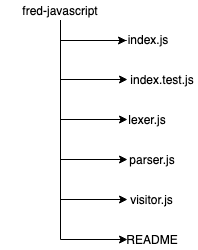
\includegraphics[keepaspectratio=true,scale=0.7]{figuras/jstree.png}
	\caption{Árvore de arquivos do projeto fred-javascript.}
	\label{fig:filetreejs}
\end{figure}

Essa implementação está publicada no npm\footnote{Node Package Manager} e possui uma
documentação simples no seu README.

\section{Suíte de Testes do FRED}

Dado a complexidade tanto de especificar como de implementar uma linguagem, nem sempre 
as implementações estão de acordo com a especificação. Para garantir que ocorra isto foi criado
uma suíte de testes da linguagem FRED, inspirada nas suítes de teste
para a linguagem TOML\footnote{\url{https://github.com/BurntSushi/toml-test}}
e Sass\footnote{\url{https://github.com/sass/sass-spec}}.

Essa suíte determina dois grupos de testes. Os que testam documentos FRED inválidos
e os que testam documentos FRED válidos.

\begin{itemize}
    \item Os testes inválidos consistem em arquivos FRED com valores inválidos para a linguagem
    e as implementações devem retornar erro quando tentar analisar esse documento.
    \item Os testes válidos consistem em arquivos de entrada com FRED válido e arquivos
    de sáida do tipo JSON, esses arquivos JSON estão num formato específico que codificam
    FRED a partir de uma transformação que não produz perda de informação.
\end{itemize}

Os arquivos de saída do tipo JSON precisam representar o documento de entrada FRED de maneira
clara e específica pois as implementações irão fazer o \textit{parsing} desta entrada e transformar
num JSON de acordo com esse formato. Portanto, especificar esse formato é extremamente importante. Um valor FRED
representado em JSON segue o seguinte padrão.

\begin{itemize}
    \item Valores FRED com tag são representados como um objeto JSON com três atributos, tag, meta, value.
    \item Valores FRED sem tag são representados da mesma maneira como em JSON se for possível, exceto objetos.
    \item Valores FRED sem tag que não existem em JSON são representados como um objeto com dois campos type e value.
    Value normalmente consiste em uma serialização do objeto como string.
    \item Objetos FRED são representados como um objeto com campo type igual a \textit{object} e no campo value
    um objeto seguindo as regras anteriores.
\end{itemize}

As tags tem seu valor representado como string e metadados são representados 
como um objeto onde a chave representa o nome do atributo FRED e o valor 
representa o valor do metadado FRED.

Exemplo de documento FRED e respectiva representação em JSON, nos códigos \ref{lst:testfred}
e \ref{lst:testjson}.

\begin{lstlisting}[caption=Exemplo de FRED ,label={lst:testfred}]
Person (source=facebook) {
    name : "Richard"
    birth-date : 1997-12-08T12:32:45Z
    age : 21
    accomplishments : [
        "high school"
        "Chess champion"
    ]
}
\end{lstlisting}


\begin{lstlisting}[caption=Exemplo de JSON no formato de testes ,label={lst:testjson}]
{
    "tag" : "Person",
    "meta" : {
        "source" : "facebook"
    },
    "value" : {
        type : "object",
        value : {
            "name" : "Richard",
            "birth-date" : {
                "type" : "date",
                "value" : "1997-12-08T12:32:45Z"
            },
            "age" : "21", 
            "accomplishments" : [
                "high school",
                "Chess champion"
            ]
        }
    }
}
\end{lstlisting}
    
Definida essa especificação, durante o trabalho foi criado um repositório onde
foram construídos vários casos de testes, sendo 25 testes para FRED válidos
e 25 para FRED inválidos.

O fluxo base para testar as implementações com esta suíte de testes é 
importar repositório de testes, ler os testes dos arquivos, criar 
casos de teste dinamicamente e executá-los.

Este fluxo foi utilizado tanto em Haskell como em JavaScript. Respectivamente
com a biblioteca hspec\footnote{\url{https://github.com/hspec/hspec}} e 
jest\footnote{\url{https://github.com/facebook/jest}}.
Ambas possuem uma API muito parecida e criar os testes dinamicamente segue 
um algoritmo parecido.

A suíte de testes está descrita no 
repositório \url{https://github.com/fred-format/fred-test}

\section{Análise de performance}

A linguagem FRED foi construída pensando tanto na facilidade para ler e escrever, como na
simplicidade para construir \textit{parsers}. Também possui abstrações que permitem incluir
mais significado semântico aos dados e, no futuro, incluir sistemas de validação e conversão
automática de tipo. 

O FRED foi desenvolvido pensando em alguns casos de uso. Inicialmente a linguagem
tem o uso principal para troca de dados, comunicação entre sistemas e
outras formas de representação de dados que devem ser legíveis para seres humanos
como arquivos de configuração.

Outro uso interessante é a facilidade de representar árvores sintáticas em FRED.
Pois, devido as tags \textit{union types} são facilmente representadas 
e portanto construir uma árvore sintática fica simples como no exemplo
\textbf{Mul [\$x, Add [40, 2]]}.

Essa representação possui vantagens em relação as \textit{S-expressions}, que
é uma notação utilizada para representar listas aninhadas e árvores, popular em linguagens da família 
LISP. Visto que, o papel do nó da árvore é destacado e possui um local natural para a 
inclusão de meta-informação.

Essa seção discute as principais características de performance da linguagem. E também como ela 
se relaciona com outros formatos, especialmente JSON e XML. É difícil avaliar 
aspectos subjetivos como legibilidade e precisão. Por isso vamos focar em uma métricas fácil de 
analisar que é o tamanho dos documentos, além disso essa medida é fundamental em sistemas 
que se comunicam por uma rede distribuída para diminuir a latência de comunicação.

\subsection{Comparação com JSON e XML}

FRED e JSON se assemelham porém o FRED possui uma notação especial
relacionada as tags e metadados. O XML por construção, entretanto tem uma 
sintaxe totalmente diferente baseada no SGML, que é uma linguagem de marcação e não de
representação de dados.

Os cenários utilizados para a coleta das métricas, foram desenvolvidos
baseados em três casos de uso que visam abranger de maneira imparcial
as notações comparadas.

O primeiro cenário atinge a representação de dados em comunicação  
entre sistemas, o outro cenário abrange representação de HTML e documentos
de marcação e por fim o último cenário foi focado em representar arquivos de configuração que 
provavelmente são escritos e lidos por humanos.

Os documentos utilizados para comparação e coleta de métricas estão no Apêndice \ref{sec:docsexamples}.
Foram retiradas métricas relacionadas a quantidade de caracteres e bytes. Para tal, utilizou-se a seguinte
metodologia:

\begin{itemize}
    \item As métricas foram calculadas a partir de três exemplos representados 
    de maneira mais similar possível em cada formato.
    \item Para calcular a quantidade de caracteres e bytes utilizou-se o comando \textit{wc}.
    \item As métricas foram calculadas tanto nos documentos puros como nos minificados e 
    comprimidos, para minificar foi utilizado minificadores simples que trabalham apenas 
    com identação e espaços em branco. A forma de compressão foi Zip e Brotli.
\end{itemize}

Retirar as métricas em arquivos comprimidos é importante, pois o tráfego de dados feito
com o protocolo HTTP é normalmente comprimido.

Para o primeiro cenário foi analisado as lingugens XML, JSON e FRED quando representando dados
utilizados em comunicação entre sistemas. Foi criado um cenário onde é representado 
uma pessoa em uma rede social. Como no exemplo \ref{lst:personexfred}.

\begin{lstlisting}[caption=Exemplo de dado sobre uma pessoa ,label={lst:personexfred}]
Person (source=facebook) {
    name : "Richard"
    birth-date : 1997-12-08T12:32:45Z
    age : 21
    accomplishments : [
        "high school"
        "Chess champion"
    ]
}
\end{lstlisting}

As métricas foram coletadas sobre os documentos \ref{lst:personxml}, \ref{lst:personjson} e
\ref{lst:personfred} que estão no Apêndice \ref{sec:docsexamples}. Os resultados estão 
na Tabela \ref{tbl:persondocs}. 

\begin{table}[h]
    \centering
	\caption{Tabela com as métricas de tamanho em bytes}
	\label{tbl:persondocs}
    \begin{tabular}{cccc}
        \toprule
        \multicolumn{1}{c}{\textbf{Tipo do Arquivo}} & \multicolumn{3}{c}{\textbf{Tamanho do Arquivo (bytes)}} \\
        \midrule
                                                     & \textbf{FRED} & \textbf{JSON} & \textbf{XML}    \\
        \midrule
        Puro              & 1331       & 2077 (156\%) & 1732 (130\%) \\
		Minificado        & 703 (53\%) & 801  (113\%) & 1127 (160\%) \\
        Minificado Zip    & 463 (34\%) & 473  (102\%) & 490  (106\%) \\
        Minificado Brotli & 243 (18\%) & 253  (104\%) & 265  (109\%) \\
		\bottomrule
    \end{tabular}
\end{table}

O documento puro significa o texto identado e com todos os espaços em branco.
O minificado passou por um processo de retirar caracteres desnecessários visando
diminuir o tamanho do arquivo. Por fim a compressão foi feita usando duas técnicas
Zip e Brotli. 

Para o segundo cenário, está sendo representado um arquivo HTML. Com isto, podemos avaliar
como as linguagens comportam-se em relação a marcação de texto. Para tal,
foi utilizado no FRED uma notação parecida com o exemplo \ref{lst:divexfred}.

\begin{lstlisting}[caption=Exemplo de dado representando HTML,label={lst:divexfred}]
div (class="card") [
    h1 "Card h1"
    h2 "Card h2"
    ul [
        li "Element 1"
        li "Element 2"
    ]
]
\end{lstlisting}

As métricas foram coletadas nos documentos \ref{lst:divxml}, \ref{lst:divjson},
\ref{lst:divfred} que estão no Apêndice \ref{sec:docsexamples} 
e os resultados estão na Tabela \ref{tbl:divdocs}.

\begin{table}[h]
    \centering
	\caption{Tabela com as métricas de tamanho em bytes}
	\label{tbl:divdocs}
    \begin{tabular}{cccc}
        \toprule
        \multicolumn{1}{c}{\textbf{Tipo do Arquivo}} & \multicolumn{3}{c}{\textbf{Tamanho do Arquivo (bytes)}} \\
        \midrule
                                                     & \textbf{FRED} & \textbf{JSON} & \textbf{XML}    \\
        \midrule
        Puro  & 789 & 6503 (824\%) & 919 (116\%)\\
		Minificado & 497 (63\%) & 1575 (317\%) & 628 (126\%) \\
        Minificado Zip & 290 (37\%) & 359 (124\%) & 314 (108\%) \\
        Minificado Brotli & 127 (16\%) & 178 (140\%) & 139 (109\%) \\
		\bottomrule
    \end{tabular}
\end{table}

Vale ressaltar que a representação em JSON utiliza a forma como a biblioteca React
representa a DOM pois é o mais próximo de um consenso pragmático
de como representar HTML em JSON.

Por fim, foi desenvolvido um cenário que abrange documentos provavelmente
lidos e escritos por humanos, no caso arquivos de configuração. Para o 
FRED foi utilizado a notação como em \ref{lst:packageexfred}.

\begin{lstlisting}[caption=Exemplo de documento para arquivo de configuração ,label={lst:packageexfred}]
{
    name : "node-js-sample"
    version : "0.2.0"
    main : "index.js"
    scripts : {
        start : "node index.js"
        test : "node index.test.js"
    }
}
\end{lstlisting}

As métricas foram coletadas sobre os documentos \ref{lst:packagexml}, \ref{lst:packagejson} e 
\ref{lst:packagefred} que estão no Apêndice \ref{sec:docsexamples}.
Os resultados estão na Tabela \ref{tbl:packagedocs}. 

\begin{table}[h!]
    \centering
	\caption{Tabela com as métricas de tamanho em bytes}
	\label{tbl:packagedocs}
    \begin{tabular}{cccc}
        \toprule
        \multicolumn{1}{c}{\textbf{Tipo do Arquivo}} & \multicolumn{3}{c}{\textbf{Tamanho do Arquivo (bytes)}} \\
        \midrule
                                                     & \textbf{FRED} & \textbf{JSON} & \textbf{XML}    \\
        \midrule
        Puro  & 611 & 646 (106\%) & 755 (124\%) \\
		Minificado & 423 (69\%) & 457 (108\%) & 611 (144\%) \\
        Minificado Zip & 458 (75\%) & 466 (102\%) & 501 (109\%)\\
        Minificado Brotli & 256 (42\%) & 255 (99\%) & 278 (109\%) \\
		\bottomrule
    \end{tabular}
\end{table}

É necessário utilizar documentos maiores para avaliar as formas de compressão entre
Zip e Brotli. Visto que o \textit{header} do Zip parece ser bem maior que o de 
Brotli.

A linguagem FRED foi mais compacta em todos os casos e talvez seja mais legível, entretanto
como exposto anteriormente é difícil retirar métricas sobre características subjetivas 
de linguagens.